\chapter{Value of the project: the influence of the number of innovation jumps}
\label{chapter:max}



%%%%%%%%%%%%%%%%%%%%%%%%%%%%%%%%%%%%%%%%%%%%%%%%%%%%%%%%%%%%%%%%%%%%%%%%
\section{Introduction}
\label{section:max_intro}

Previous chapters were focused on a timeline starting at the instant a desired innovation level $\theta$ was achieved and hence, ignoring all what happened before it. Following this reasoning we 
studied the value function and the demand value that triggers the investment associated to three different contexts: entering the market with an innovative product; introducing a new product with the immediate replacement of the \textit{old} one; introducing of a \textit{new} product with the possibility of immediate replacement of the \textit{old} one or simultaneous production followed by the replacement of the \textit{old} product).
% -, by setting time to start when
% while considering a fixed level of innovation $\theta$.

On this chapter we are interested
%to calculate the maximized expected value function, associated to each of the three contexts,
in the calculation of the value function with respect to the R\&D investment, taking into account the waiting time until the innovation breakthrough takes place.
This allows us to state a relation between the R\&D investment and the time a firm needs to wait until it is in a favourable situation to invest.
%give a weight depending on the time we need to wait until we are able to introduce the \textit{new} product.

%Here we will consider the case when $\theta$ is achieved at the next jump and, the generalization of it, when only at the $n$-th jump ($n \in \mathds{N}$) we obtain the desired threshold $\theta$.


Innovation levels are assumed to increase by jumps. Therefore the innovation process
%As stated in Introduction, recall that the innovation process 
$\Theta=\{ \theta_t, \ t \geq 0 \}$ is defined as an homogenous Compound Poisson Process, with constant rate given by $\lambda(R)=R^\gamma$, with $R$ corresponding to the investment in the R\&D department, and $\gamma$ a sensitivity parameter taking values in $(0,1]$.

%The higher the R\&D investment, the smaller the expected waiting time until the desired level $\theta$ occurs is, so the higher the value function will be.

Note that R\&D investment (R) is different from investment costs ($\delta K$): the first influences directly the innovation $\Theta$, while the second is related with costs the firm needs to incur to adapt its production to the new technology level.
For example, R\&D costs can be related with scientist wages and laboratory equipment, while investment costs can be related with new equipment the firm needs to purchase or formation necessary to its employees, in order to adapt to the new technology.



The innovation process can be then expressed as
$$\theta_t=\theta_0+uN_t, \ t\geq 0.$$ 
with $\theta_0$ denoting the state of technology at the initial point in time, $u>0$ a fixed jump size and $\{ N_t, \ t \geq 0 \}$ the jump process which follows a Poisson Process with rate $\lambda(R)$. 
%Note that the higher the innovation threshold $\theta$ desired, the later the innovation will occur (in average), but the higher the demand for the \textit{new} product will be.

Considering now $S_n$ to be the random variable that represents the waiting time until the $n$-th jump in the process is observed, accordingly to \cite{ross}, $S_n$ follows an Erlang distribution with shape parameter $n$ and rate parameter $\lambda(R)$, the same as in the jump process, that is,
$$S_n=\min \{t\geq 0: N(t)=n \} \sim Erlang(n,\lambda(R)).$$

It immediately follows that the expected waiting time for the $n$-th jump to be reached is given by $\mathds{E}(S_n)=\frac{n}{\lambda(R)}$, meaning that the larger the R\&D investment, the sooner the $n$-th jump is expected to happen. Also, note that, if there is no investment on R\&D, the jumps are supposed to occur at a null rate ($\lambda(0)=0$), resulting in a infinite expected waiting time. In fact, when $\lambda(0)=0$, we assume that the technology level does not change and therefore our problem is ill-posed. For this reason, we assume that $\lambda(R)>0$.
%Accordingly to \cite{ross}, we have that $S_n$ is distributed according to Erlang distribution with shape parameter $n$ and rate parameter being the same as the Poisson Process, that is, $\lambda(R)$. From this it follows that the expected waiting time for the $n$-th jump to be reached is given by $\mathds{E}(S_n)=\frac{n}{\lambda(R)}.$ Thus, the higher the investment, the bigger the quantity of jumps observed is. Note that, in the situation in which there is no R\&D investment, there is also no evolution in the innovation process, since it implies a null rate $\lambda(0)=0$ followed by an infinite waiting time for any amount of jumps wanted to be observed.

%Note from previous deduced expressions of value function that none of them depend on the R\&D investment $R$. This one only influences the innovation process. Therefore, as it will be showed in the next sections, this is a standard maximization problem, in which we will want to maximize the expected value function with respect to the R\&D investment $R$.
% the work made in the last chapter of \cite{rita}, since our investment decision is not done based on a certain optimal innovation level, but, instead, based on optimal demand level(s), only after a threshold innovation level $\theta$ is reached.



In this chapter we are interested to study how the complete value of the project - reflecting R\&D investment so as the innovative product investment - is affected by the R\&D investment and the number of jumps needed until it is favourable to invest on the innovative product. First we focus on the situation when the innovation breakthrough happens within one innovation jump and then we generalise this scenario, by considering the breakthrough to occur within $n\in\mathds{N}$ jumps.


We close this introduction highlighting the fact that every investment value function previously deduced is independent of the R\&D investment, depending solely on the technology level $\theta$.

%%%%%%%%%%%%%%%%%%%%%%%%%%%%%%%%%%%%%%%%%%%%%%%%%%%%%%%%%%%%%%%%%%%%%%%%
\section{One jump}
\label{section:max_1jump}

We start with the simplest case: the desired innovation level $\theta$ is reached within one jump.
Therefore $S_1$ denotes the random variable associated to the waiting time until the jump occurs and it is such that
$$S_1 \sim \text{Erlang}(1,\lambda(R)) \overset{d}{=} \text{Exponential}(\lambda(R)).$$

We also denote by $F$ the value function associated to an investment situation and $V$ to be the maximized value of the investment project given by
\begin{equation}
	V(x)=\max_R \mathds{E} [ e^{-rS_1}F(x)-R]\geq 0
	\label{max_V}
\end{equation}

It consists on the maximized expected value of the investment on a new technology minus R\&D costs associated. Note that, since we assumed the timeline of $F$ to start when the innovation breakthrough occurs ($S_1$), we discount its value to the time the R\&D investment is made and consider $x$ to be the demand value expected to observe at $S_1$.

Here we assume, which notoriously leads to a simpler analysis, that no matter when the innovation breakthrough happens, the level of the process $X$ is deterministic and given by $x$.

%Note that, having calculated $F$, all terms are deterministic with the exception of the waiting time until the breakthrough occurs. Therefore, we need to calculate the expected value of the whole investment.
%and corresponding to the maximized expected discounted value function minus the R\&D investment needed to be made. Recall that, in the previous sections, we deduced all the value functions by setting the initial time to be the time at the innovation threshold $\theta$ is reached. Therefore in order to have the real value, we need to discount it to the time when the jump happens, that is, $S_1$. Also, since the jumps are governed by a stochastic process (and thus they are random), we need to calculate the expected value of the discounted value function. Since the R\&D investment $R$ is deterministic, it could be inside or outside the expected value (but for the sake of simplicity we decided to include it when calculating the expectation).

%In order to estimate the function $V$, one could have made it directly through stochastic simulations, using Monte Carlo methods for instance. However we here we deduced an analytical result, which is stronger than any estimation made.
%preferred to deduce an analytical result, since its stronger than any estimation made. 

We note that although $F$ results from an optimal stopping problem, $V$ is a (standard) optimization problem w.r.t. a deterministic value $R$, denoting the R\%D costs.

Taking into account that the expectation is with respect to $S_1$, we obtain
%Coming back to the expression of $V$ in \eqref{max_V}, and by considering the expectation with respect to $S_1$ we obtain that it follows
\begin{align}
 V(x)&=\max_R  \left\{ \int_0 ^\infty f_{S_1}(t) e^{-rt} F(x) dt -R \right\} \nonumber \\
 &=\max_R  \left\{ \int_0 ^\infty \lambda(R) e^{-\lambda(R)t} e^{-rt} F(x) dt -R \right\} \label{max_V2}
\end{align}
where $f_{S_1}$ corresponds to the probability density function of an Exponential distribution with parameter $\lambda(R)$. %, associated to the random variable $S_1$.

As previously written (and deduced), none of the value functions studied depends on the R\&D investment or on the time at they are evaluated, only on the demand level observed at the breakthrough. $F$ never depends on $R$ or $t$. Therefore the integral on \eqref{max_V2} can be solved, leading to
\begin{equation}
V(x)=\max_R \left\{ \frac{\lambda(R)}{\lambda(R)+r} F(x) -R \right\}=\max_R \left\{ \frac{R^\gamma}{R^\gamma+r} F(x) -R \right\},
\label{max_V3}
\end{equation}
which is a maximization problem with respect to the R\&D investment $R$. Since by \eqref{max_V}, $V$ cannot be negative it follows that the restriction
\begin{equation}
R^\gamma F(x) - (R^\gamma+r)R \geq 0 \ \Leftrightarrow  F(x) \geq \frac{R^\gamma+r}{R^{\gamma-1}}
	\label{max_rest}
\end{equation}
must always be verified.

%The optimal value of the investment to be made, from now on denoted by $R^*$, is found by analyzing the first and the second partial derivatives of the expression to maximize, that is,
Thus the following standard optimization technique is used to find $V$:
\begin{align}
\frac{\partial}{\partial R} \left( \frac{R^\gamma}{R^\gamma+r} F(x) -R \right) &= \frac{\gamma R^{\gamma-1}F(x)r-(R^\gamma+r)^2}{(R^\gamma+r)^2} \label{max_ddR}\\
\frac{\partial^2}{\partial R^2} \left( \frac{R^\gamma}{R^\gamma+r} F(x) -R \right) &=
-\frac{F(x) \gamma r R^{-2+\gamma}(r-\gamma r+(1+\gamma)R^\gamma)}{(R^\gamma+r)^3}\leq 0.
\label{max_d2dR2}
\end{align}

Note that, since $\gamma \in (0,1]$, $F(x)\geq0, \ \forall x$ and $r, \ R >0$, the second partial derivative with respect to $R$ \eqref{max_d2dR2} is always negative. Hence the expression to be maximized in \eqref{max_V3} corresponds to a concave function, meaning that we are always able to find a value $R^*=\arg \underset{R}{\max} \left\{ \frac{R^\gamma}{R^\gamma+r} F(x) -R \right\}$.

Therefore $R^*$ is such that \ref{max_ddR}, computed at $R^*$ is zero. Then it follows that $R^*$ depends intrinsically on $\gamma$, and so, next we analyse its effects.

%Regarding the set of possible values for $\gamma$ and their interest, we consider two different cases.

%Firstly we analyse the solution considering $\gamma=1$, meaning that jumps happen at a rate equal to the investment made. This is the only case for which

%we were able to obtain an analytical solution. Secondly we analyse other possible values $\gamma \in (0,1)$, whose results are only able through a numerical solver and software \texttt{Mathematica}.

%The case $\gamma=0$ is not here considered due to its lack of relevance for the problem.
% , regarding the problem in hands. Note that 
%Since $\gamma=0 \ \Rightarrow \ \lambda(R)=1,$ the innovation rate is not influenced by the R\&D investment made.

%that is, considering $\gamma=0$, the innovation rate is not influenced by the size of the R\&D investment made (which is not compatible with the real life).

$\bullet$ \textbf{Case I:} $\gamma=1 \Leftrightarrow \lambda(R)=R$

First of all, note that this case means that jumps occur at a rate given precisely by the investment costs.

Analysing the roots of the first partial derivative in order to investment parameter $R$, we get a quadratic polynomial, whose zeros are given by
%which we can calculate obtain the expression of the zeros, obtaining
%$$   \frac{\partial}{\partial R} \left( \frac{R}{R+r} F(X) -R \right) = \frac{ F(X)r-(R+r)^2}{(R+r)^2}=0 $$
%$$   \Rightarrow F(X)r-(R^2+2rR+r^2)=0$$
$$  R=-\sqrt{F(x)r}-r \  \vee \ R=\sqrt{F(x)r}-r$$

Since it is not possible to have negative investment, we discard the leftmost solution.
%The first solution is not admissible, since it's not possible to have negative investment ($R>0$).

The second solution is admissible, since it is always true that
\begin{align}
 \sqrt{F(x)r}-r  \ &\underset{\eqref{max_rest}}{\geq} \ \sqrt{(R+r)r}-r \geq 0 \nonumber \\
 &\Leftrightarrow rR+r^2-r^2=rR\geq 0.
 %= \sqrt{rR+R^2}-r  \ \underset{\triangle}{\geq} \ \sqrt{rR}+\sqrt{R^2}-r=\sqrt{rR},
\end{align}

%On account of the negativity 
%Concerning the second partial derivative \eqref{max_d2dR2}, we obtain that, if \eqref{max_rest} holds, then the optimal R\&D investment to be made corresponds to
Thus, if condition \eqref{max_rest} holds, the optimal investment is given by
\begin{equation}
R^*=\max_R V(x)= \sqrt{F(x)r}-r.
\end{equation}


$\bullet$ \textbf{Case II:} $\gamma \in (0,1) $

Considering now $\gamma \in (0,1) $ and taking into account expression \eqref{max_ddR}, potential maximizers of $V$, %stationary points 
will be found by calculating the roots of the following polynomial
\begin{equation}
R^{\gamma-1}F(x)r-R^{2\gamma}-2rR^\gamma-r^2=0.
 \label{max_root}
\end{equation}


From condition \eqref{max_d2dR2} it follows that the maximizer $R^*$ is such that it verifies \eqref{max_rest} and \eqref{max_root}.

Unfortunately, we are not able to solve \eqref{max_root} analytically for any value $\gamma \in (0,1) $. However, using software \texttt{Mathematica}, we performed some numerical illustrations for values $\gamma \in (0,1)$, presented in Section \ref{maximexp_cs}.


\section{Multiple jumps}
\label{section:max_jumps}

Now we take another step and generalize the previous idea, by considering that the desired innovation level $\theta$ is reached at the $n$-th innovation jump.
Therefore we consider $S_n$ to be the random variable associated to the waiting time until the $n$-th jump occurs and it is such that
$$S_n \sim \text{Erlang}(n,\lambda(R)).$$

Note that by considering $n=1$, we are at the situation analysed in the previous section.

For the sake of simplicity we keep the same notation as before, where $F$ denotes the value function associated to a certain investment situation and $V$ the maximized expected discounted value function minus the R\&D investment needed to be made, is now given by
\begin{align}
V_n(x)&=\max_R \mathds{E} [ e^{-rS_n}F(x)-R] \nonumber \\
&=\max_R  \left\{ \int_0 ^\infty f_{S_n}(t) e^{-rt} F(x) dt -R \right\} \nonumber \\
&=\max_R  \left\{ \int_0 ^\infty \frac{\lambda(R)^n t^{n-1}}{(n-1)!} e^{-\lambda(R)t} e^{-rt} F(x) dt -R \right\}
\label{max_2V}
\end{align}
where $f_{S_n}$ corresponds to the probability density function of an Erlang with shape parameter $n$ and rate parameter $\lambda(R)$.
%, associated to the random variable $S_n$.

Considering $W$ to be a random variable such that $W \sim \text{Erlang}(n, \lambda(R)+r)$ and $f_W$ the correspondent probability density function, the integral above can be simplified as follows
\begin{align}
\int_0 ^\infty \frac{\lambda(R)^n t^{n-1}}{(n-1)!} e^{-\lambda(R)t} e^{-rt} F(x) dt &=
\frac{\lambda(R)^n}{(\lambda(R)+r)} F(x) \int_0 ^\infty \frac{(\lambda(R)+r)^n t^{n-1}}{(n-1)!} e^{-t(\lambda(R)+r)} dt \nonumber \\
&=\left( \frac{\lambda(R)}{\lambda(R)+r}\right)^n F(x)  \int_0 ^\infty f_W(t) \ dt \nonumber \\
&=\left( \frac{\lambda(R)}{\lambda(R)+r}\right)^n F(x). \label{max_2V2}
\end{align}

Plugging the resulting expression \eqref{max_2V2} in \eqref{max_2V}, we obtain that $V_n$ corresponds to a standard maximization problem given by
\begin{equation}
V_n(x)=\max_R \left\{ \left( \frac{\lambda(R)}{\lambda(R)+r}\right)^n F(x)-R \right\}=\max_R \left\{ \left( \frac{R^\gamma}{R^\gamma+r}\right)^n F(x)-R \right\}.
	\label{max_2V3}
\end{equation}

Since $V_n$ is expected to be greater or equal to 0 $\forall n \in \mathds{N}$, the following restriction must hold
\begin{align}
R^{\gamma n} F(x)-R(R^\gamma + r)^n \geq 0 \  \Leftrightarrow \ F(x) \geq \frac{(R^\gamma+r)^n}{R^{\gamma n -1}}.
\label{max_2rest}
\end{align}


%The optimal investment to be made, considering that at the $n$-th jump we achieve the desired breakthrough level $\theta$ and from now on denoted by $R^*_n$, is found by analysing the first and the second partial derivatives of the expression to maximize, that is,
Then the optimal investment in R\&D centres, $R^*$, should be such that the following holds:
\begin{align}
\frac{\partial}{\partial R} \left( \left( \frac{R^\gamma}{R^\gamma+r}\right)^n F(x)-R \right) &= \frac{\gamma  F(x) n r \left(\frac{R^{\gamma }}{r+R^{\gamma }}\right)^n-r R+R^{\gamma +1}}{r R+R^{\gamma +1}}=0 \label{max_2ddR}\\
\frac{\partial^2}{\partial R^2} \left( \left( \frac{R^\gamma}{R^\gamma+r}\right)^n F(x)-R\right) &=
\frac{\gamma  F(x) n r \left(\frac{R^{\gamma }}{r+R^{\gamma }}\right)^n \left(r (\gamma  n-1)-(\gamma +1) R^{\gamma }\right)}{R^2 \left(r+R^{\gamma }\right)^2}<0.
\label{max_2d2dR2}
\end{align}

Due to the complexity of both expressions above represented, we are not able to deduce an expression for stationary points neither to assess if the second partial derivative is negative. And, consequently, we need to resort to numerical calculations.


Although, here we do not present a complete study for it, these calculations are quite easy to implement, in order to find an approximation of $R^*$ with respect to several values of the parameter $\gamma$. In this view, we developed the function \texttt{V} presented on Appendix \ref{chapter:appendixjump}.
%Thus stationary points are numerically calculated. If, when evaluated at \eqref{max_2d2dR2}, they return a negative value, they are relative maximums (otherwise they are relative minimums on which we are not interested). The optimal investment $R^*$ is selected among all relative maximums as the one which maximizes $V_n$.
%This time we are not able to deduce if the second partial derivative is negative. Thus, in order to check if a stationary point is a minimum or a maximum, we will replace its value on expression \eqref{max_2d2dR2}. If it leads to a negative value, it will be considered as a relative maximum. $R^*$ will be selected among all these values to be one that maximizes the most $V_n$.

%We are not even able to find any stationary point analytically, due to the complexity of \eqref{max_2ddR}.













\section{Comparative Statics}
\label{maximexp_cs}

In this Section we assess how optimal investment ($R^*$), its associated rate jump ($\lambda(R^*)$) and optimal value function ($V_n$) behave with the number of jumps considered ($n$) and sensitivity chosen ($\gamma$).


Since we are not abe to deduce any analytical expression regarding the optimal R\&D investment, we develop a function that returns an approximation to the optimal R\&D investment, for a fixed situation. This function is presented in Appendix \ref{chapter:appendixjump} and it is named \texttt{calcR}.

In view of the numerical experiments, by the independence of $F$ on parameters $R$ and $\gamma$, we consider it to be fixed and to take the value of 10. The discount rate is fixed at $r=0.05$ and $\gamma$ is considered to start at $0.05$ and incremented $0.05$ until it reaches 1.

%As stated in Section \ref{section:max_jumps}, we are not able to find an analytical expression regarding the roots of expression \eqref{max_2ddR} and hence we are not able to derive ana analytical expression for the optimal R\&D investment $R^*$. However, we developed a function that, given a certain parameter $\gamma$ and an amount of jumps $n$ and considering a fixed discount rate $r$ and the value function evaluated for an initial demand level $x$ $F(x)$, calculates numerically the R\&D investment that optimizes expression \eqref{max_ddR}, that leads to function $V_n$. This function is presented in Appendix by the name \texttt{calcR}. All of the next results were obtained using it.

%%The following parameters were considered regarding all the next results:
%\begin{itemize}
%	\item $r=0.05$;
%	\item $F(X)=10$;
%\end{itemize}
%We also considered different values of $\gamma \in (0,1]$, starting in 0.05 and, incremented by 0.05, until 1.

%Note on expression \eqref{max_2V3}, since $F(x)$ is not influenced by $\gamma$ or $R$, it can be seen as a constant term representing the value of the project assuming an innovation level $\theta$, which is yet to come. Hence we are able to proceed with our numerical approximations.

We start analysing the case when a firm is in a favourable position to invest after an innovation jump (this is the case when $n=1$).

\begin{figure}[!htb]
	\begin{subfigmatrix}{2}
		\subfigure[$R \in {(0,1]} $ and $\gamma \in {(0,1]} $. ]{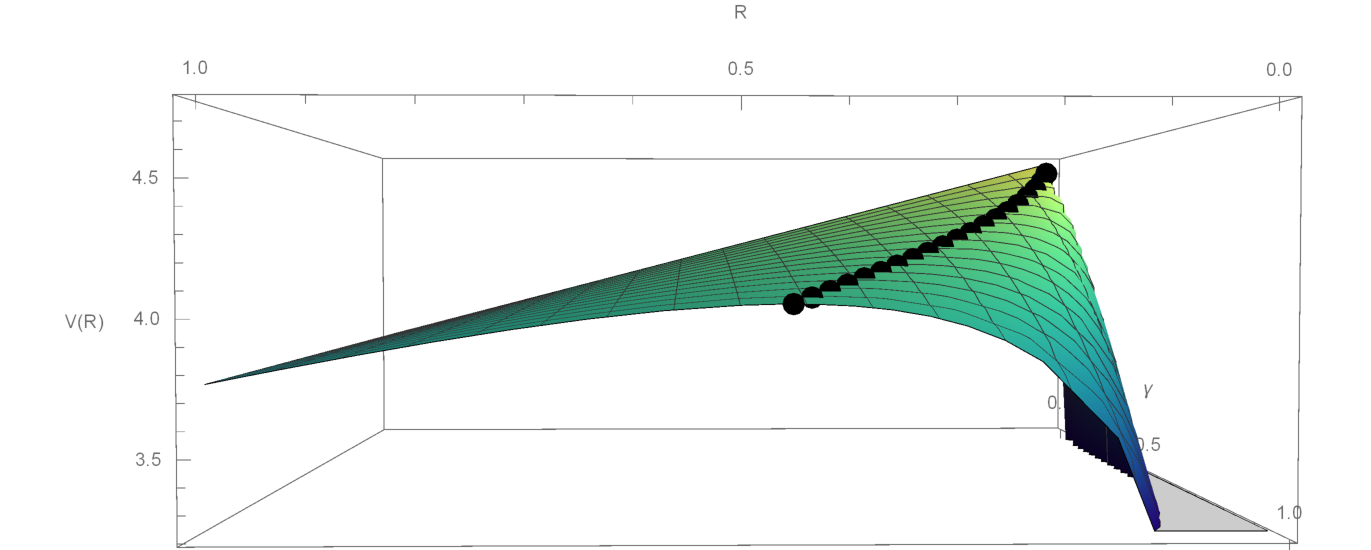
\includegraphics[width=0.45\textwidth]{Jumps/RgammaV.pdf}}
		\subfigure[A particular case: $\gamma=0.5$.
		]{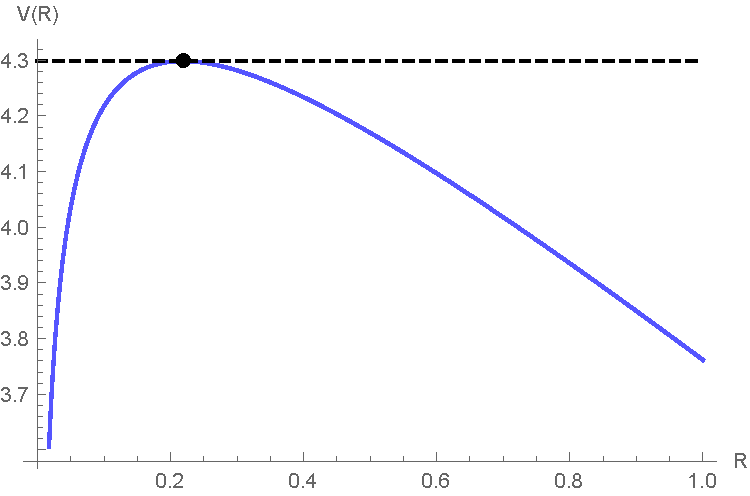
\includegraphics[width=0.45\textwidth]{Jumps/RVgamma5.pdf}}
	\end{subfigmatrix}
	\caption{Function to be maximized in \eqref{max_V} with respect to parameters $\gamma$ and $R$ and corresponding maximum values $V_1$ regarding each $\gamma$ (black)}
	\label{fig:max_n1}
\end{figure}

On Figure \ref{fig:max_n1} (a) we observe that the function to be maximized is concave with respect to the R\&D investment $R$. This seems to be related with the balance achieved between the linear decay of $V$ with the R\&D investment made and the greater jump rate and, consequently, sooner expected level of innovation, and smaller discount weight on $F$, both influenced by the investment $R$. 
Furthermore, we observe the smaller the $\gamma$, the larger optimal R\&D investment $R^*$ is.


%This seems to be related with the fact that a smaller $\gamma$ leads to higher jump rate, which implies a higher expected time. Thus, to balance this increasing on the expected waiting time, one increases the R\&D investment.

On Figure \ref{fig:max_n1} (b) it is illustrated the particular case when $\gamma=0.5$ and the associated optimal R\&D investment (corresponding to 4.3). %For $n=1$ we are able to obtain all $R^*$, but same doesn't hold for bigger values of $n$.

Now we increase the complexity and analyse the behaviour of $R^*$, $\lambda(R^*)$ e $V_n$, regarding the occurrence of 1 to 5 innovation jumps.

\begin{figure}[!htb]
	\begin{subfigmatrix}{2}
		\subfigure[3D view. ]{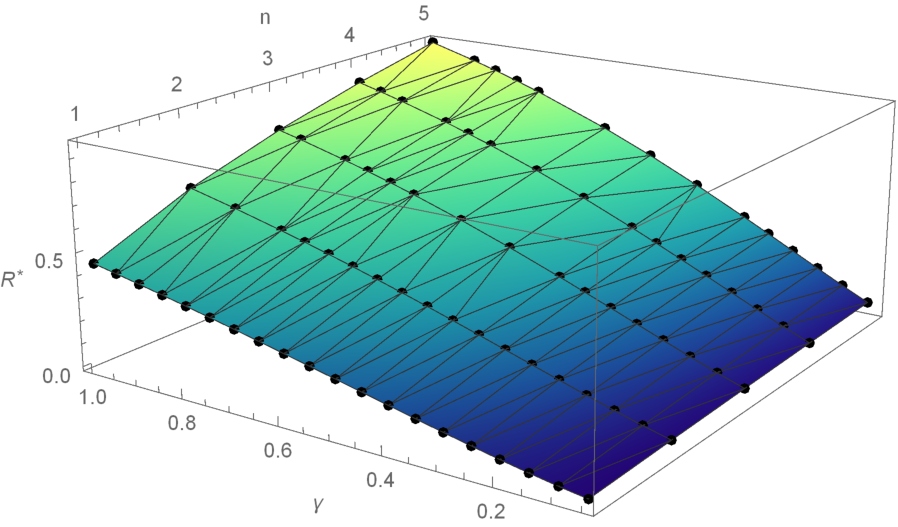
\includegraphics[width=0.45\textwidth]{Jumps/gammanR.pdf}}
		\subfigure[2D view.
		]{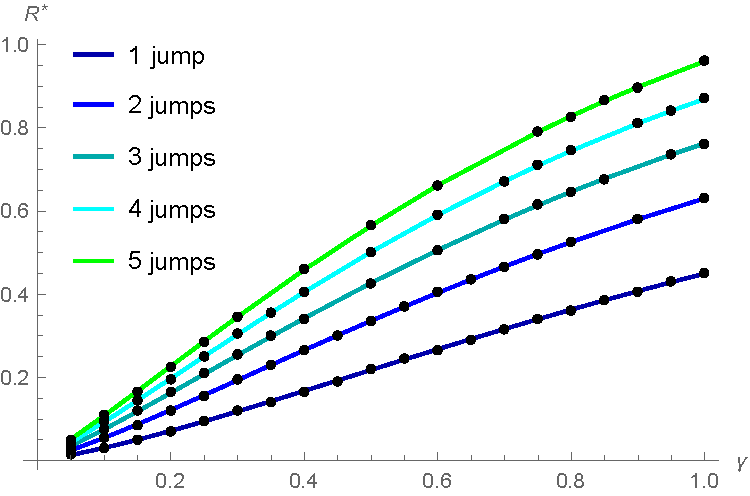
\includegraphics[width=0.45\textwidth]{Jumps/jump.pdf}}
	\end{subfigmatrix}
	\caption{Optimal R\&D values $R^*$ regarding parameter $\gamma$ and the occurrence of $n\in \{1,...,5\}$ innovation jumps, with corresponding numerical approximations (black). }
	\label{fig:max_nR}
\end{figure}

On the grounds of the results shown on Figure \ref{fig:max_nR}, we conclude that the optimal R\&D investment increases with both sensitivity $\gamma$ and number of jumps $n$. Note it is not possible to obtain the optimal value $R^*$ (for instant for $\gamma=0.45$ and $n\geq 3$). However using the values obtained in their neighbourhood, we are able to estimate its tendency, as represented on both figures \ref{fig:max_n1} and \ref{fig:max_nR}.
%by connecting the values that we were able to calculate, we are able to check the (mentioned) increasing tendency.

\begin{figure}[!htb]
	\begin{subfigmatrix}{2}
		\subfigure[Jump rate $\lambda(R^*)$. ]{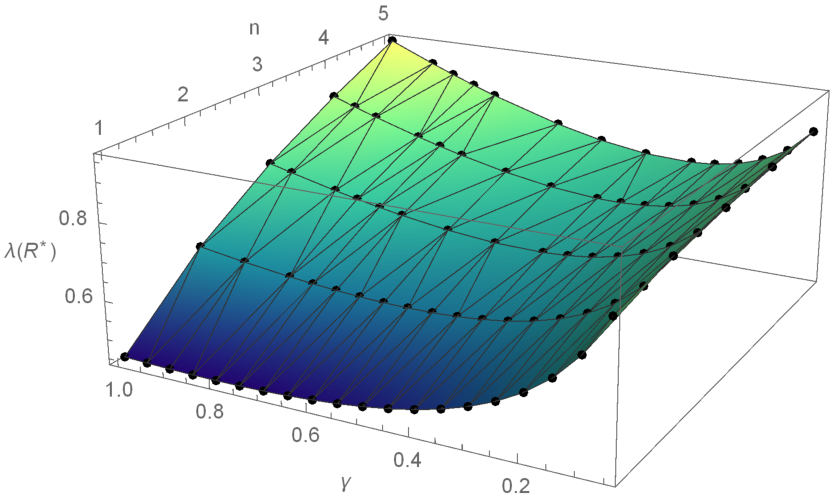
\includegraphics[width=0.45\textwidth]{Jumps/gammanlambda.pdf}}
		\subfigure[$V_n$
		]{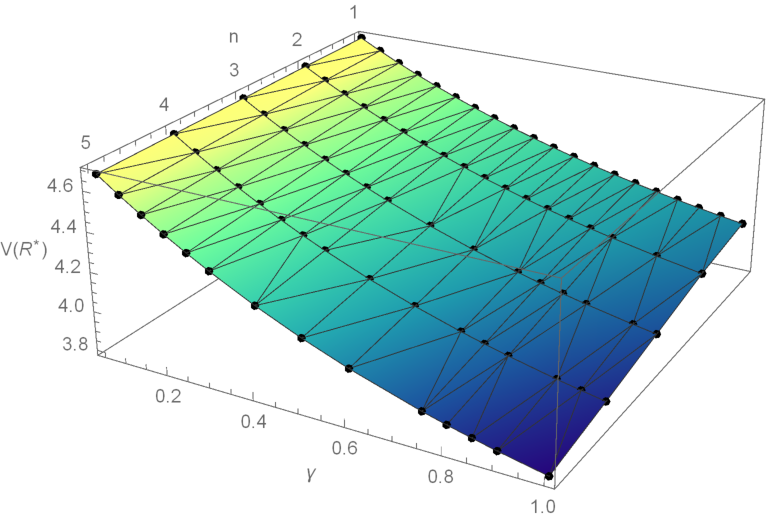
\includegraphics[width=0.45\textwidth]{Jumps/gammanV.pdf}}
	\end{subfigmatrix}
	\caption{Effect of parameters $\gamma$ and the occurrence of $n\in \{1,...,5\}$ innovation jumps on jump rate $\lambda(R^*)$ and project's value $V_n$, with corresponding numerical approximations (black). }
	\label{fig:max_n}
\end{figure}


We observe on Figure \ref{fig:max_n} (a) that the jump rate $\lambda(R^*)$ increases with the number of jumps considered $n$. However, the same does not hold for parameter $\gamma$: we observe that the jump rate has a non-monotonic behaviour with $\lambda$, a consequence of the exponentiation $R^\gamma$.

%We suspect this is related with the optimal value $R^*$ and its exponentiation with $\gamma$, necessary to calculate $\lambda(R^*)$.


Figure \ref{fig:max_n} (b) shows that the non-monotonic behaviour of $\lambda(R^*)$ seems not to influence (strongly) the tendency of $V_n$, since $V_n$ decreases with both $n$ and $\gamma$.

We propose that the higher the number of jumps until the firm is able to invest, the greater is the amount of time the firm is expected to wait to be in a favourable position to invest, leading to a larger discount on the value function $F$ and, therefore, to a smaller value of the project $V$. 
On the other side, the larger the sensitivity $\gamma$, the larger the optimal investment $R^*$ and the smaller the jump rate. This leads to a project with comparative smaller value.


%The first is explained due to the fact that if the higher the number of jumps we need to wait, before being able to think about the investment, the lower is the value of the project we have in hands (when compared with one of same value $F$ and same parameter $\gamma$).